\documentclass[a4paper,openright,12pt]{book}

\usepackage[spanish]{babel}
\usepackage[utf8]{inputenc}
\usepackage{enumerate}
\usepackage{url}
\usepackage{graphicx}
\graphicspath{ {./img/} }
\usepackage{wrapfig}
\usepackage{a4wide}
\usepackage{html}
\usepackage{hthtml}
\usepackage{listings}
\usepackage{multirow}
\usepackage{lscape}

\usepackage[font={footnotesize,it}]{caption}
\usepackage[normalsize]{subfigure}
\usepackage{color}
\usepackage[usenames,dvipsnames,svgnames,table]{xcolor}
\usepackage{amsmath}

\pretolerance=10000
%Para que no corte las palabras al final de la linea.

\DeclareGraphicsExtensions{.png,.jpg,.pdf,.eps}
\usepackage{geometry}
\geometry{a4paper, left=2.6cm, right=2.2cm, top=3.0cm, bottom=3.0cm}

\linespread{1.3}

\setlength{\parskip}{1ex plus 0.5ex minus 0.2ex}

%listings style
\definecolor{mygreen}{rgb}{0,0.6,0}
\definecolor{mygray}{rgb}{0.5,0.5,0.5}
\definecolor{mymauve}{rgb}{0.58,0,0.82}
\definecolor{lightgray}{rgb}{.9,.9,.9}
\definecolor{darkgray}{rgb}{.4,.4,.4}
\definecolor{purple}{rgb}{0.65, 0.12, 0.82}

\lstset{
	language=xml,
	tabsize=3,
	label=code:sample,
	frame=shadowbox,
	rulesepcolor=\color{gray},
	xleftmargin=20pt,
	framexleftmargin=15pt,
	keywordstyle=\color{blue}\bf,
	commentstyle=\color{OliveGreen},
	stringstyle=\color{red},
	numbers=left,
	numberstyle=\tiny,
	numbersep=5pt,
	breaklines=true,
	showstringspaces=false,
	basicstyle=\footnotesize,
	emph={model, name, static, link, pose, collision, geometry, mesh, scale, uri, visual},emphstyle={\color{magenta}}
}

\begin{document}
	
	
	
	
	
	
% Para que salga la bibliografia en el indice
\let\OLDthebibliography=\thebibliography
\def\thebibliography#1{\OLDthebibliography{#1}%
	\addcontentsline{toc}{chapter}{\bibname}}

\tableofcontents
\listoffigures
	
	
\chapter{Introducción}
\label{ch:Introduccion}

En este proyecto se construirán escenarios para la enseñanza utilizando diversas tecnologías. Para poder saber cual es el marco de desarrollo y donde se engloban los conceptos utilizados vamos a introducir algunos términos que servirán como contexto y que nos permitirán entender mejor de dónde surje la necesidad de estos escenarios y cuall es la utilidad de los mismos.

\section{Robótica}
\label{sec:intr_robotica}

Según la Wikipedia\cite{wikipedia}, \textit{La robótica es la rama de la ingeniería mecatrónica, de la ingeniería eléctrica, de la ingeniería electrónica, de la ingeniería mecánica, de la ingeniería biomédica y de las ciencias de la computación que se ocupa del diseño, construcción, operación, disposición estructural, manufactura y aplicación de los robots.}

Otra definición menos técnica podría ser: La robótica es una ciencia o rama de la tecnología, que estudia el diseño y construcción de máquinas capaces de desempeñar tareas realizadas por el ser humano o que requieren del uso de inteligencia. Por tanto, estamos ante una ciencia que se encarga de diseñar máquinas que sean capaces de reemplazar al ser humano en algunas acciones. Es una disciplina con sus propios problemas, sus fundamentos y sus leyes, y podemos observar dos vertientes de la misma, la teórica y la práctica. En la parte teórica podemos agrupar todas las aportaciones de la informática, la intenligencia artificial y la automatización. En cuanto a la parte práctica observamos aportaciones relativas tanto a la construcción del robot como a la de su gestión, siendo por tanto destacadas las aportaciones de la mecánica, electrónica, programación, etc. Esto hace de la robótica una ciencia con un marcado carácter interdisciplinario.

\subsection{Historia de la robótica}
\label{subsec:intr_historiarobotica}

La historia de la robótica ha estado unida a la construcción de “artefactos”, que trataban de materializar el deseo humano de crear seres semejantes a nosotros que nos descargasen del trabajo. Desde los primeros pasos de la civilización el ser humano ha desarrollado ingenios tanto para facilitar sus labores como para imitar a la naturaleza, fascinando a sus congéneres. De los antiguos egipcios se conservan descripciones de más de 100 máquinas y autómatas, incluyendo un artefacto con fuego, un órgano de viento, una máquina operada mediante una moneda, una máquina de vapor, en la obra \textit{Pneumática y Autómata} de Herón de Alejandría. Los griegos nos dejaron creaciones como un pájaro de madera, a vapor, que fue capaz de volar, y genios como Leonardo da Vinci el diseño de un \textit{Caballero mecánico}. 

\begin{wrapfigure}{r}{0.3\textwidth}
	\centering
	\includegraphics[width=0.2\textwidth]{pato.jpg}
	\caption{Pato con aparato digestivo de Jacques de Vaucanson.} \label{fig:pato}
\end{wrapfigure}
El francés Jacques de Vaucanson creó en el siglo XVIII lo que se consideran los primeros robots de la historia: El flautista, El tamborilero y el Pato con aparato digestivo (\textit{Figura \ref{fig:pato}}). También creó el primer telar completamente automático del mundo. Unos años más tarde, Joseph Jacquard inventa en 1801 una máquina textil programable mediante tarjetas perforadas, y Henri Maillardert construyó una muñeca mecánica que era capaz de hacer dibujos. Al mismo tiempo, en Japón, se creaban juguetes mecánicos que sirven té, disparan flechas y pintan. Podemos considerar esta época el nacimiento de los robots tal como los conocemos actualmente.

En el año 1921 un escritor checo, Karel Capek, publica su obra \textit{“Los Robots Universales de Rossum”}, en la que aparece por primera vez la palabra “robot“ derivada de la palabra checa robota, que significa servidumbre o trabajo forzado. Unos años más tarde, en 1942, la revista americana \textit{Astounding Science Fiction} pública "Círculo Vicioso" (Runaround en inglés), una historia de ciencia ficción escrita por Isaac Asimov donde aparecen por primera vez las Tres leyes de la robótica. Estas leyes establecen lo siguiente:
\begin{quote}
\begin{enumerate}[1.ª]
	\item Un robot no hará daño a un ser humano o, por inacción, permitir que un ser humano sufra daño.
	\item Un robot debe hacer o realizar las órdenes dadas por los seres humanos, excepto si estas órdenes entrasen en conflicto con la 1ª Ley.
	\item Un robot debe proteger su propia existencia en la medida en que esta protección no entre en conflicto con la 1ª o la 2ª Ley.
\end{enumerate}
\end{quote}

Pese a que son fruto de una obra de ciencia ficción, estas leyes han dado la vuelta al mundo y multitud de científicos e investigadores las toman como ciertas, siendo un concepto que aún hoy tiene sentido para los futuros desarrollos en torno a sistemas autónomos. La autonomía de las máquinas debería acompañarse de medidas de seguridad que evitaran el daño a las personas. Esto es un precepto que las tres leyes de la robótica de Asimov contienen. De hecho, la idea del escritor era proteger al ser humano, que los robots, por muy avanzados que estuvieran, no pudieran volverse contra las personas. En el caso de un coche autónomo, si este conduce sin pasajeros dentro y va a chocar contra otro donde viajan varias personas, ¿debe el primer vehículo echarse a un lado aunque esté circulando correctamente y vaya a sufrir más daños si lo hace? La primera ley de Asimov diría que sí. En cuanto a la segunda ley, actualmente no se concibe el desarrollo de ningún sistema autónomo sin mecanismos que permitan a las personas manejarlos manualmente, y se considera que aún no existe un sistema tan fiable y preciso como para darle mayor autoridad que al ser humano que lo controla. Evidentemente un sistema autónomo hará todo lo posible para no sufrir daños. Como toda tecnología, está diseñada para que funcione y para que mantenga su integridad y su funcionamiento. Su duración será mayor o menor dependiendo de la calidad, pero desde luego no acometerá operaciones destinadas a estropearse. En el año 1982 Isaac Asimov publicó \textit{El robot completo} (The Complete Robot en inglés), una colección de cuentos de ciencia ficción escritos entre 1940 y 1976. En esta colección vuelve a explicar las tres leyes de la robótica con más ahínco y complejidad moral. Incluso llega a plantear la muerte de un ser humano por la mano de un robot con las tres leyes programadas, por lo que decide incluir una cuarta ley "La ley 0 (cero)": \textit{Un robot no hará daño a la Humanidad o, por inacción, permitir que la Humanidad sufra daño}.

\begin{wrapfigure}{l}{0.3\textwidth}
	\centering
	\includegraphics[width=0.2\textwidth]{unimation.jpg}
	\caption{Robot de Unimation usado por Ford en 1961.} \label{fig:unimation}
\end{wrapfigure}
En la década de 1950 se comienzan a desarrollar los primeros robots comerciales, nacidos de las patentes de la década anterior. Debido a la investigación en inteligencia artificial se encontraron maneras de emular el procesamiento de información humana con computadoras electrónicas y se desarrollaron una variedad de mecanismos para probar estas teorías. En 1956 se comercializa el primer robot de la compañía Unimation, fundada por George Devol y Joseph Engelberger. En 1961 se instala en una fábrica de la Ford Motors Company uno de estos robots (\textit{Figura \ref{fig:unimation}}), cuya función era la de levantar y apilar grandes piezas de metal caliente. En 1971 el “Standford Arm“, un pequeño brazo robótico de accionamiento eléctrico, se desarrolló en la Standford University. En 1973 la empresa Kuka\footnote{\url{https://www.kuka.com/}} desarrolla el primer robot industrial con seis ejes electromecánicos, el Famulus. Unos años más tarde, en 1975, la empresa Unimation comercializó un brazo manipulador programable universal llamado PUMA.

Pero la robótica no se basa sólo en las máquinas que revolucionaron los procesos industriales, el concepto de robótica incluye y cada vez se orienta más hacia los sistemas móviles autónomos, que son aquellos capaces de desenvolverse por sí mismos en entornos desconocidos sin necesidad de supervisión. Con esta idea en mente, en los setenta, la NASA inicio un programa de cooperación con el Jet Propulsión Laboratory para desarrollar plataformas capaces de explorar terrenos hostiles. El primer fruto de esta alianza sería el Mars-Rover (\textit{Figura \ref{fig:marsrover}}), que estaba equipado con un brazo mecánico tipo Standford, un dispositivo telemétrico láser, cámaras estéreo y sensores de proximidad. Sin embargo, fue la Unión Soviética en 1971 la primera en aterrizar un robot en la superficie de marte con éxito, el Mars 3, aunque la comunicación se perdió minutos después. No fue hasta 1976 que la NASA hizo llegar al primer robot estadounidense a Marte, el Viking I. En la Figura \ref{fig:vikingmars} podemos observar ambos robots.

\begin{figure}[t]
	\centering
	\subfigure[Mars 3]{\includegraphics[width=0.4\textwidth]{mars3.jpg}}\hspace{0.05\textwidth}
	\subfigure[Viking I]{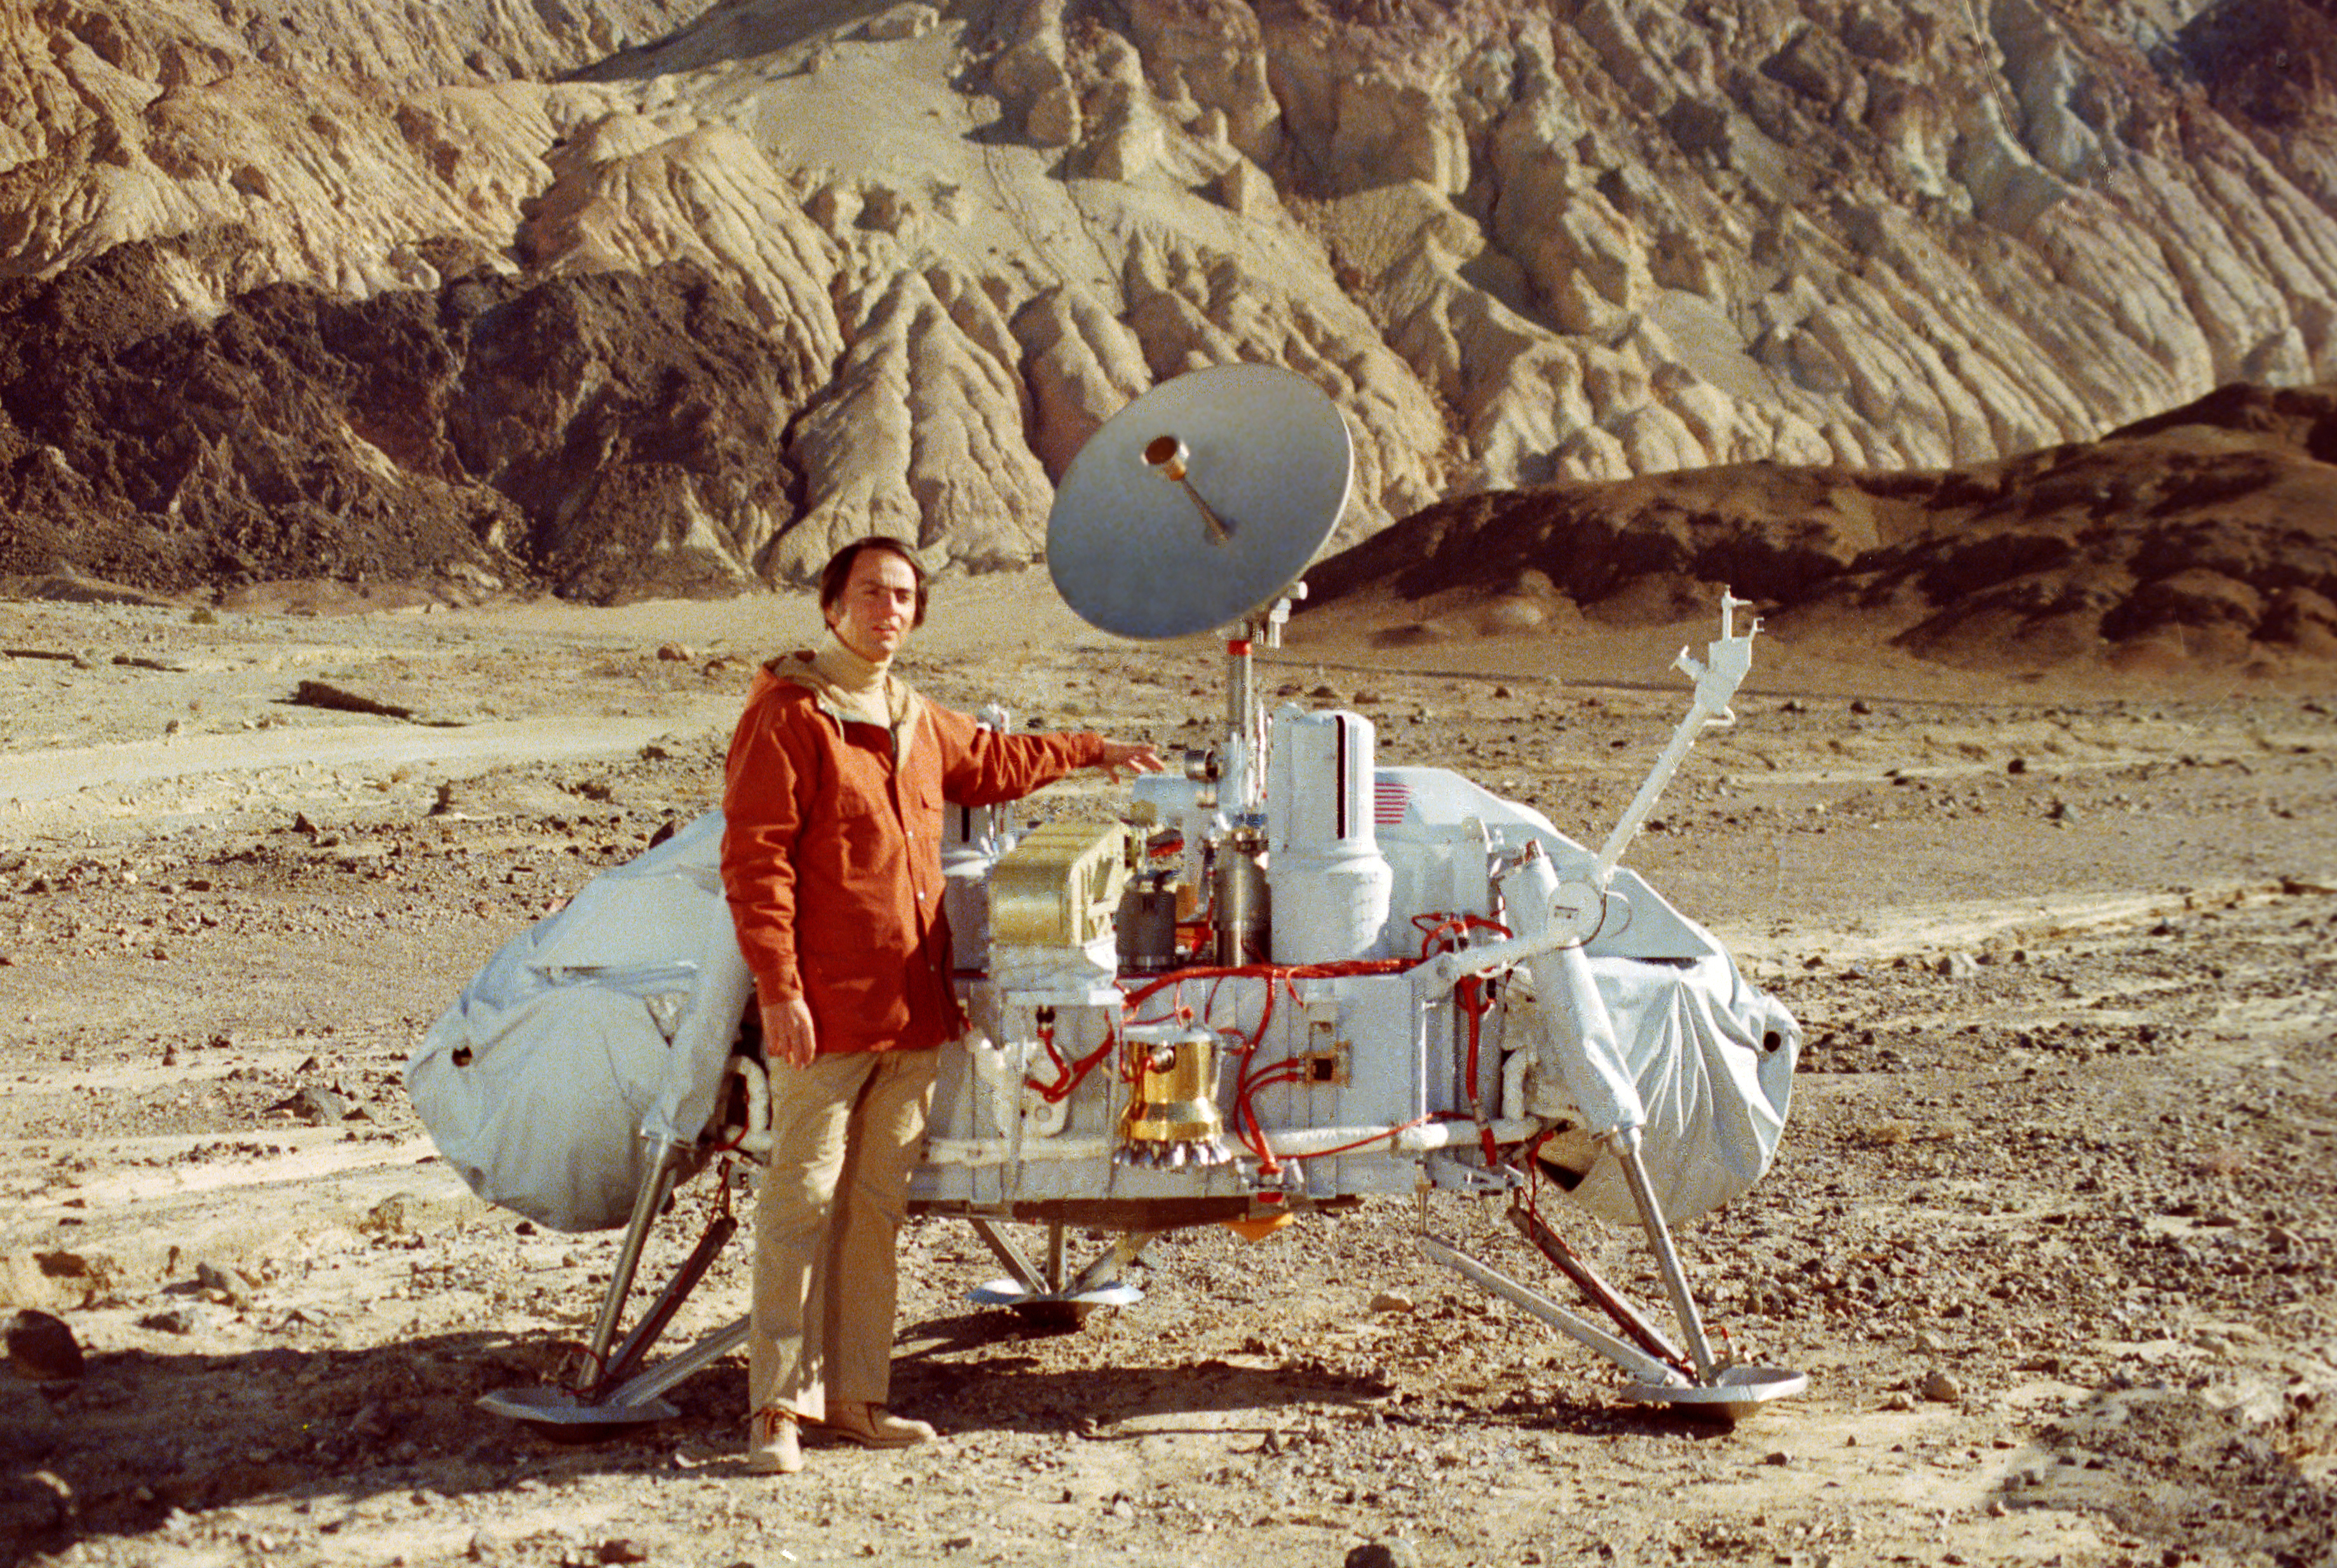
\includegraphics[width=0.4\textwidth]{viking1.jpg}}
	\caption[Los primeros robots espaciales, el Mars 3 y el Viking I]{Imágenes de los primeros robots espaciales: una copia del Mars 3 (a) expuesto en el Museo Memorial de la Cosmonáutica en Moscú, y en Dr. Carls Sagan posando junto a un modelo del Viking I (b) en el Valle de la Muerte, California} \label{fig:vikingmars}
\end{figure}

Desde entonces la robótica ha experimentado en multitud de aplicaciones y formatos con modelos sumamente ambiciosos, como es el caso del IT, diseñado para expresar emociones, el COG, tambien conocido como el robot de cuatro sentidos, el famoso Sojourner (\textit{Figura \ref{fig:marsrover}}) o el Lunar Rover, vehículo con control remoto, y otros mucho mas específicos como el Cypher, un helicóptero robot de uso militar, el guardia de trafico japonés Anzen Taro o los robots mascotas de Sony. En el campo de los robots antropomorfos (androides) se debe mencionar el P3 de Honda que mide 1.60m, pesa 130 Kg y es capaz de subir y bajar escaleras, abrir puertas, pulsar interruptores y empujar vehículos, así como el robot ASIMO de la misma compañía, capaz de desplazarse de forma bípeda e interactuar con las personas.

En la Figura \ref{fig:marsrover} podemos observar la evolución de los robots usados en la exploración espacial, pues se encuentran tres generaciones de Mars Rover de la NASA. Abajo en el centro nos encontramos con el primer Mars Rover, el Sojourner, que aterrizó en Marte en 1997 como parte del proyecto Mars Pathfinder Project. Es el más pequeño de los tres, con 65 centímetros de largo. A la izquierda se encuentra un vehículo de pruebas MER (Mars Exploration Rover), que mide en torno a los 1.6 metros de largo. Éste es un gemelo operativo del Spirit y del Oportunity que aterrizaron en la superficie marciana en 2004. A la derecha se encuentra un Rover de pruebas, de unos 3 metros de largo, del Laboratorio de Ciencia de Marte (Mars Science Laboratory), responsables del aterrizaje del Curiosity en Marte en 2012.

\begin{figure}[t]
	\centering
	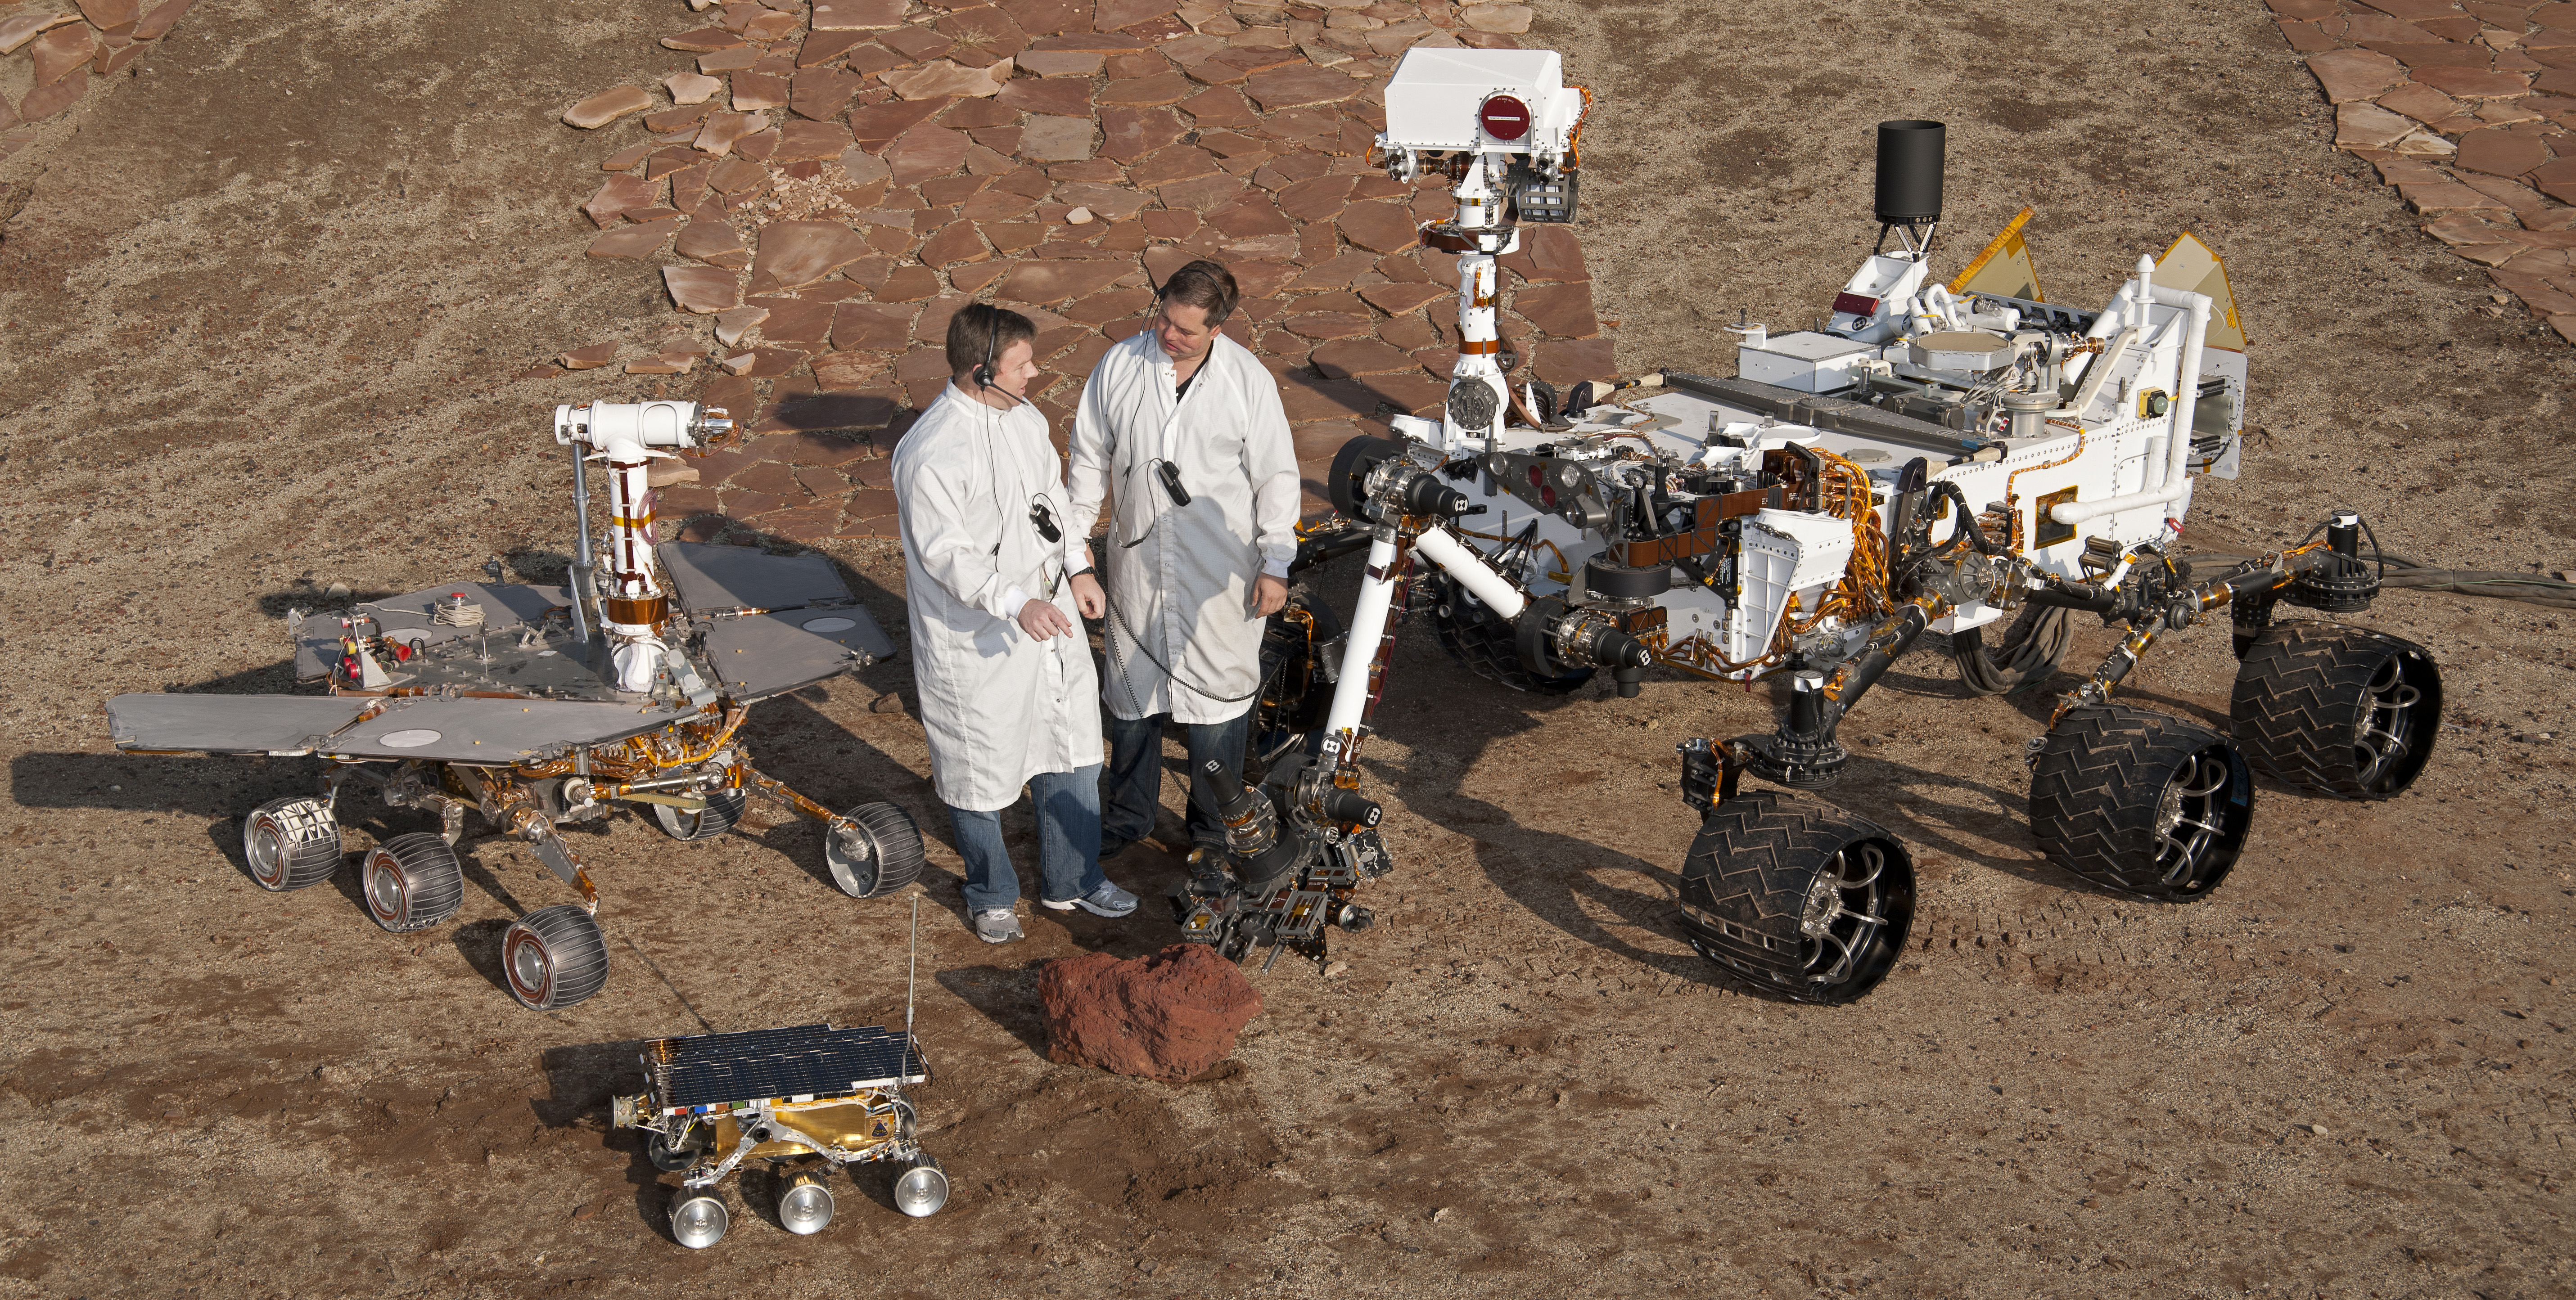
\includegraphics[width=0.8\textwidth]{marsrover.jpg}
	\caption{Dos ingenieros de la Nasa posan con tres generaciones de Mars Rovers.} \label{fig:marsrover}
\end{figure}

En general la historia de la robótica la podemos clasificar en cinco generaciones (división hecha por Michael Cancel, director del Centro de Aplicaciones Robóticas de Science Application Inc. en 1984): 
\begin{enumerate}[1.ª Generación]
	\item[1.ª Generación] Robots manipuladores. Son sistemas mecánicos multifuncionales con un sencillo sistema de control, bien manual, de secuencia fija o de secuencia variable.
	\item[2.ª Generación] Robots de aprendizaje. Repiten una secuencia de movimientos que ha sido ejecutada previamente por un operador humano. El modo de hacerlo es a través de un dispositivo mecánico. El operador realiza los movimientos requeridos mientras el robot le sigue y los memoriza.
	\item[3.ª Generación] Robots con control sensorizado. El controlador es una computadora que ejecuta las órdenes de un programa y las envía al manipulador para que realice los movimientos necesarios.
	\item[4.ª Generación] Robots inteligentes. Son similares a los anteriores, pero además poseen sensores que envían información a la computadora de control sobre el estado del proceso. Esto permite una toma inteligente de decisiones y el control del proceso en tiempo real.
\end{enumerate}

Las dos primeras, ya fueron alcanzadas en los ochenta. La tercera generación, que incluye visión artificial, ha avanzado mucho en los ochenta y noventas. La cuarta contempla movilidad avanzada en exteriores e interiores. Y podríamos hablar incluso de una quinta, en la cual entrarían los más modernos sistemas de aprendizaje autónomo y la inteligencia artificial.

Otra clasificación muy extendida de los robots es según su estructura. La estructura está definida por el tipo de configuración general del Robot. El concepto de metamorfismo, de reciente aparición, se ha introducido para incrementar la flexibilidad funcional de un Robot a través del cambio de su configuración por el propio Robot. El metamorfismo admite diversos niveles, desde los más elementales (cambio de herramienta o de efecto terminal), hasta los más complejos como el cambio o alteración de algunos de sus elementos o subsistemas estructurales. Los dispositivos y mecanismos que pueden agruparse bajo la denominación genérica del Robot, tal como se ha indicado, son muy diversos y es por tanto difícil establecer una clasificación coherente de los mismos que resista un análisis crítico y riguroso. La subdivisión de los Robots, con base en su arquitectura, se hace en los siguientes grupos: 
\begin{enumerate}[1.]
	\item Poliarticulados. En este grupo se encuentran los Robots de muy diversa forma y configuración, cuya característica común es la de ser básicamente sedentarios (aunque excepcionalmente pueden ser guiados para efectuar desplazamientos limitados) y estar estructurados para mover sus elementos terminales en un determinado espacio de trabajo según uno o más sistemas de coordenadas, y con un número limitado de grados de libertad. En este grupo, se encuentran los manipuladores, los Robots industriales, los Robots cartesianos y se emplean cuando es preciso abarcar una zona de trabajo relativamente amplia o alargada, actuar sobre objetos con un plano de simetría vertical o reducir el espacio ocupado en el suelo. Econtramos un ejemplo de robot poliarticulado de la empresa Sepro\footnote{\url{http://www.sepro-group.com/es}} en la Figura \ref{fig:poliarticulado}.
	\begin{figure}[h]
		\centering\includegraphics[width=0.4\textwidth]{robotpoliarticulado.jpg}
		\caption{Robot poliarticulado de la empresa Sepro.}
		\label{fig:poliarticulado}
	\end{figure}
	
	\item Móviles. Son Robots con gran capacidad de desplazamiento, basados en carros o plataformas y dotados de un sistema locomotor de tipo rodante. Siguen su camino por telemando o guiándose por la información recibida de su entorno a través de sus sensores. Estos Robots aseguran el transporte de piezas de un punto a otro de una cadena de fabricación. Guiados mediante pistas materializadas a través de la radiación electromagnética de circuitos empotrados en el suelo, o a través de bandas detectadas fotoeléctricamente, pueden incluso llegar a sortear obstáculos y están dotados de un nivel relativamente elevado de inteligencia. Podemos ver un ejemplo de robot móvil en la Figura \ref{fig:movil}.
	\begin{figure}[h]
		\centering\includegraphics[width=0.45\textwidth]{robotmovil.jpg}
		\caption{Robot androide.}
		\label{fig:movil}
	\end{figure}	

	\item Androides. Son los tipos de Robots que intentan reproducir total o parcialmente la forma y el comportamiento cinemático del ser humano. Actualmente, los androides son todavía dispositivos muy poco evolucionados y sin utilidad práctica, y destinados, fundamentalmente, al estudio y experimentación. Uno de los aspectos más complejos de estos Robots, y sobre el que se centra la mayoría de los trabajos, es el de la locomoción bípeda. En este caso, el principal problema es controlar dinámica y coordinadamente en el tiempo real el proceso y mantener simultáneamente el equilibrio del Robot. Podemos ver el robot Nao\footnote{\url{http://aliverobots.com/nao/}} en la Figura \ref{fig:androide}, un ejemplo de robot androide de la empresa Robotrónica\footnote{\url{http://aliverobots.com/}}, una división de la empresa Juguetrónica\footnote{\url{https://www.juguetronica.com/}}. 
	\begin{figure}[h]
		\centering\includegraphics[width=0.25\textwidth]{robotandroide.jpg}
		\caption{Robot androide Nao.}
		\label{fig:androide}
	\end{figure}

	\item Zoomórficos. Los Robots zoomórficos, que considerados en sentido no restrictivo podrían incluir también a los androides, constituyen una clase caracterizada principalmente por sus sistemas de locomoción que imitan a los diversos seres vivos. A pesar de la disparidad morfológica de sus posibles sistemas de locomoción es conveniente agrupar a los Robots zoomórficos en dos categorías principales: caminadores y no caminadores. El grupo de los Robots zoomórficos no caminadores está muy poco evolucionado. Los experimentos efectuados en Japón basados en segmentos cilíndricos biselados acoplados axialmente entre sí y dotados de un movimiento relativo de rotación. Los Robots zoomórficos caminadores multípedos son muy numerosos y están siendo objeto de experimentos en diversos laboratorios con vistas al desarrollo posterior de verdaderos vehículos terrenos, pilotados o autónomos, capaces de evolucionar en superficies muy accidentadas. Las aplicaciones de estos Robots serán interesantes en el campo de la exploración espacial y en el estudio de los volcanes. Podemos ver varios ejemplos de robots zoomórficos en la Figura \ref{fig:zoomorficos}.
	\begin{figure}[h]
		\centering
		\subfigure[Robot perro]{\includegraphics[width=0.4\textwidth]{robotperro.jpg}}\hspace{0.04\textwidth}	
		\subfigure[Robot araña]{\includegraphics[width=0.4\textwidth]{robotarana.png}}\vspace{0.03\textwidth}
		\subfigure[Robot pez]{\includegraphics[width=0.4\textwidth]{robotpez.jpg}}\hspace{0.04\textwidth}
		\subfigure[Robot serpiente]{\includegraphics[width=0.4\textwidth]{robotserpiente.png}}
		\caption[Diferentes ejemplos de robots zoomórficos]{Ejemplos de robots zoomórficos: un robot con forma de perro (a), uno con forma de araña (b), uno con forma de pez (c) y uno con forma de serpiente (d)} \label{fig:zoomorficos}
	\end{figure}
	
	\item Híbridos.	Estos Robots corresponden a aquellos de difícil clasificación, cuya estructura se sitúa en combinación con alguna de las anteriores ya expuestas, bien sea por conjunción o por yuxtaposición. Por ejemplo, un dispositivo segmentado articulado y con ruedas, es al mismo tiempo, uno de los atributos de los Robots móviles y de los Robots zoomórficos. Podemos ver un ejemplo de robot híbrido en la Figura \ref{fig:hibrido}, en este caso uno de los muchos utilizados para desactivar o explosionar bombas de forma controlada por las fueras de seguridad y policía de numerosos países.
	\begin{figure}[h]
		\centering\includegraphics[width=0.35\textwidth]{robothibrido.jpg}
		\caption{Robot híbrido usado en la desactivación de bombas.}
		\label{fig:hibrido}
	\end{figure}
\end{enumerate}


\section{La robótica en la enseñanza}
\label{sec:intr_roboticaensenanza}

El campo de la robótica está en constante expansión, y su popularidad aumenta rápidamente. Ya no solo vemos grandes avances en los robots industriales, como en cadenas de producción, envasado de alimentos o gestión de almacenes, sino que los robots domésticos están cobrando cada vez más importancia. El éxito de los robots aspiradora como Roomba de iRobot\footnote{\url{http://www.irobot.es/}}, la incorporación de aparcamiento automático en coches o incluso asistentes de conducción autónoma como el autopiloto de Tesla\footnote{\url{https://www.tesla.com/es_ES/}} o prototipos de Google o Apple, termostatos inteligentes como el Nest\footnote{\url{https://nest.com/thermostat/meet-nest-thermostat/}} de Google, o la inmensa variedad de drones del mercado ponen de manifiesto que ésta es una tendencia en auge a nivel global.

Uno de los factores que permiten diseñar, construir y comercializar este tipo de robots asegurando una inteligencia y robustez ante situaciones reales es la programación que hay detrás de estos, su software. Usualmente este software tiene varias capas (drivers, middleware y aplicaciones) y presenta unos requisitos específicos dependiendo de las funciones del robot. En los últimos años se han logrado añadir en la fabricación de estos robots ordenadores personales o microprocesadores, principalmente de bajo coste, y sistemas operativos generalistas, lo que permite aumentar la complejidad de sus tareas y el uso de herramientas estándar de desarrollo.


Este sector es un mercado al alza, que demanda científicos e ingenieros de robótica y visión artificial, pero dado que es un campo transversal los profesionales de este sector deben poseer sólidos conocimientos de programación, procesado de imágenes, calculo, álgebra lineal, métodos numéricos, electrónica y electricidad, etc. Esto hace que se puedan realizar aproximaciones desde diferentes puntos de vista. Uno de ellos, más tradicional, es desde las ingenierías eléctricas y electrónicas. La enseñanza desde estas áreas se centra en la construcción del robot, sus partes móviles y mecánicas, sus sensores, motores, su diseño electrónico, procesadores, etc. Otro acercamiento se realiza desde la Informática, poniendo más énfasis en la programación, dado que la inteligencia del robot una vez construido reside en su software.

Actualmente en nuestro país, la robótica aparece en los cursos de secundaria, aunque se realiza en la universidad con algunos títulos de grado y postgrado específicos. En la enseñanza secundaria la robótica permite acercar la tecnología a los niños y motivarles para aprender conceptos básicos de ciencias, tecnología, ingeniería y matemáticas. Estas áreas han visto reducido el número de estudiantes en los últimos años, y numerosos gobiernos han realizado grandes inversiones para incentivar a los estudiantes a orientar sus estudios hacia estos campos. En la Comunidad de Madrid se ha introducido\footnote{Decreto 48/2015} la asignatura \textit{Tecnología, programación y robótica} en el curriculum oficial de la ESO (Educación Secundaria Obligatoria). En esta etapa se utilizan plataformas como los diferentes robots de LEGO\footnote{Lego posee toda una gama pensada para la educación: \url{https://education.lego.com/}} (Mindstorms, NXT, Evo, WeDo, RCX) o placas con procesadores Arduino a las que se conectan diversos sensores, actuadores, servos, etc. Con estas plataformas se introducen las bases de la programación con lenguajes sencillos, usando entornos de prácticas donde completar código ya estructurado o entornos gráficos para niños como Scratch, RCX-code o Blockly.

La robótica genera entornos propicios para la colaboración, y el trabajo en equipo donde los niños y jóvenes tienen la oportunidad de aprender y practicar las habilidades  denominadas como las 4C del siglo XXI\footnote{Según la Asociación para las habilidades del siglo XXI (\textit{Partnership for 21st Century Skills}] \url{http://www.p21.org/}}:
\begin{itemize}
	\item Pensamiento Crítico: habilidad imprescindible para un buen aprendizaje. Se basa en la razón efectiva, utilizando varios tipos de razonamiento y anañizando la interacción de las partes de un todo, en el análisis y evaluación de las pruebas, argumentos y puntos de vista, en la interpretación de la información y extracción de conclusiones, y en la resolución de problemas.
	\item Comunicación: se basa principalmente en la articulación de pensamientos e ideas en diferentes vías, en la escucha eficaz y en el uso de múltiples medios y tecnologías.
	\item Colaboración: Se basa en la capacidad para trabajar de manera eficaz y respetuosa en diversos equipos, en la voluntad de compromiso en la consecución de objetivos comunes y en la asunción de responsabilidades, tanto compartidas como individuales.
	\item Creatividad: se basa en el pensamiento creativo, usando técnicas de generación de ideas y elaborando, perfeccionando, analizando y evaluando ideas originales, Y en el trabajo creativo, desarollando y comunicando nuevas ideas de manera efectiva, siendo abierto y receptivo a nuevas ideas y perspectivas o contribuyendo con ideas creativas en el campo de trabajo.
\end{itemize}

En la enseñanza superior o universitaria, tradicionalmente se imparten asignaturas de robótica en las escuelas de ingeniería, ya sea industrial, electrónica, informática, etc. En España existe algún grado en robótica y varios másteres. En Estados Unidos, las universidades más punteras en tecnología, como Stanford o el MIT, ya cuentan con programas de grado y postgrado entre sus planes de estudios. Las asignaturas de robótica impartidas en la universidad tienen un enfoque práctico, de forma que la interacción del alumno con los robots facilita el aprendizaje y entendimiento de los conceptos teóricos mediante un aprendizaje activo. Es habitual el uso de plataformas específicas para la programación del robot, como por ejemplo MATLAB\footnote{\url{https://es.mathworks.com/products/matlab.html}} y su paquete Simulink\footnote{\url{https://es.mathworks.com/products/simulink.html}}. Otros se centran en el diseño y modelado del robot.

\subsection{Entorno docente con JdeRobot: TeachingRobotics}
\label{subsec:intr_entornodocente}

Desde la Universidad Rey Juan Carlos se plantea un entorno de enseñanza universitaria llamado \textit{JdeRobot-TeachingRobotics}, dentro de la plataforma JdeRobot (\textit{Sección \ref{sec:plat_jderobot}}). Orientado para realizar cursos universitarios de 12-14 semanas, plantea ocultar todo el middleware al alumno y dejar que se centre en la programación de los algoritmos. De esta manera el alumno desarrolla software para una tarea determinada sin necesidad de desarrollar el software que conecta los elementos del robot, por lo que es perfecto para cursos de introducción a la robótica o que hagan énfasis en la programación de robots ya construidos. En la Universidad Rey Juan Carlos se ha utilizado en la asignatura \textquotedblleft Robótica\textquotedblright, en el grado en Ingeniería Telemática, en la asignatura \textquotedblleft Visión en Robótica\textquotedblright, en el Máster de Visión Artificial, y en varios cursos de introducción a la robótica y a los drones, así como en el campeonato PROGRAMAROBOT\footnote{\url{http://jderobot.org/Campeonato-programacion-de-robots}}.

Este entorno docente está compuesto de diferentes prácticas independientes que siguen el mismo planteamiento: se propone un problema robótico y el estudiante programa la inteligencia del robot para resolverlo. Se pueden diferenciar una serie de capas que componen dichas practicas. La capa más baja es donde se encuentra el robot, simulado o real, con todos los sensores o actuadores que lo componen. En la siguiente capa se encuentran los drivers del robot, que permiten acceder a los sensores y actuadores del robot. Y en la última capa se encuentra la aplicación, que analiza los datos de los sensores y dá órdenes a los actuadores. En esta capa se encuentra el código de toma de decisiones y planificación. Aqui se encuentra una parte de código específico y necesario para el funcionamiento del robot y otra parte en blanco que el alumno debe completar para resolver con éxito el problema planteado. 

Dichas prácticas pueden realizarse sobre robots reales o simulados, aunque generalmente es conveniente comenzar con la simulación antes de pasar a escenarios reales. Se apoyan, por tanto, en el simulador Gazebo (\textit{Sección \ref{sec:plat_gazebo}}), y usan lenguajes de programación como Python o C++. Aunque el principal sistema operativo para utilizar esta plataforma es Linux, ya sea Ubuntu o Debian, se ha usado la interfaz web de Gazebo para poder lanzarlo cómodamente en Windows y MacOS. Esto se ha conseguido lanzando el servidor de Gazebo y los drivers en un contenedor Docker, el cual permite ejecutar la aplicación de forma nativa en cada sistema operativo y conectarse mediante una aplicación web al simulador Gazebo para ver el mundo de la simulación.

Algunas de las prácticas desarrolladas son:
\begin{itemize}
	\item \textit{Drones: persecución}. En esta práctica el alumno programa un drone \textit{gato} que persigue a otro drone \textit{ratón}. El mundo de Gazebo no presenta obstáculos para facilitar la programación del robot, y los drones son similares a los AR.Drone de Parrot\footnote{\url{https://www.parrot.com/es/drones/parrot-ardrone-20-elite-edition}} (\textit{Figura \ref{fig:ardrone}}). Hay varios niveles de \textit{ratón} disponibles, cuya dificultad de persecución va en aumento. El drone \textit{gato} posee una cámara frontal, una cámara cenital, inclinómetros y GPS, y facilita una interfaz de control que acepta órdenes simples como avance hacia delante, lateral, ascenso, etc. El objetivo del estudiante es programar los elementos de percepción visual necesarios para que el drone \textit{gato} localice al drone \textit{ratón} y los movimientos necesarios para la persecución del drone \textit{ratón}. También se incluye un componente de evaluación automática y objetiva, el cual puntúa el número de segundos que la distancia con el drone \textit{ratón} está por debajo de un umbral.

\begin{figure}[h]
	\centering\includegraphics[width=0.4\textwidth]{ArDrone.png}
	\caption{Robot ArDrone en Gazebo.}
	\label{fig:ardrone}
\end{figure}
	
	\item \textit{Control visual: sigue líneas}. En esta práctica el alumno debe conseguir que un robot Kobuki (\textit{Figura \ref{fig:kobuki}}) siga la línea roja de un circuito en el menor tiempo posible. El estudiante debe realizar los filtros de percepción necesarios para que el robot siga la línea roja y los movimientos del robot para mantenerse en la trayectoria adecuada

\begin{figure}[h]
	\centering\includegraphics[width=0.4\textwidth]{kobuki.png}
	\caption{Robot kobuki en Gazebo.}
	\label{fig:kobuki}
\end{figure}
	
	\item \textit{Fórmula 1: nacegación local}. En esta práctica el alumno debe programar un coche de Fórmula 1 para que complete una vuelta a un circuito de carreras esquivando los obstáculos que se encuentre en el camino. El robot cuenta con sensores de odometría, GPS y un sensor láser, y la interfaz de movimiento admite órdenes simples como velocidad de avanze o de giro.
	
	\item \textit{TeleTaxi: navegación global}. En esta práctica el alumno debe conseguir que un coche vaya de un punto a otro cualquiera de una ciudad. El coche, taxi, tiene un sensor GPS y una interfaz como la del Fórmula 1. El alumno debe programar un algoritmo de navegación para que alcance la posición objetivo en un mapa conocido.

\begin{figure}[h]
	\centering\includegraphics[width=0.5\textwidth]{pioneer.png}
	\caption{Robot Pioneer en Gazebo.}
	\label{fig:pioneer}
\end{figure}
	
	\item \textit{Visión: reconstrucción 3D}. En esta práctica el alumno debe conseguir que un robot Pioneer (\textit{Figura \ref{fig:pioneer}}) reproduzca en 3D los elementos que se le presentan. Este robot está equipado con un par estéreo de cámaras. Para conseguir su objetivo, el alumno debe programar un algoritmo de reconstrucción 3D clásico de tres pasos: detección de puntos de interés en las dos imágenes, emparejamiento de píxeles homólogos entre ambas, y triangulación espacial para calcular el punto tridimensional que origina cada pareja de píxeles homólogos.
\end{itemize}



meter cosas de metodologia EN EL CAPITULO 2




\chapter{Infgraestructura Usada}
\label{ch:PlataformaDesarrollo}

En este capıtulo vamos a describir con más detalle todo el software utilizado en la realización del proyecto: programas, plataformas, simuladores, etc. El sistema operativo elegido para desarrollar todo el proyecto ha sido Ubuntu 16.04. Ubuntu es un sistema operativo basado en Debian GNU/Linux y que se distribuye como software libre, el cual incluye su propio entorno de escritorio denominado Unity. El nombre de la distribución proviene del concepto zulú y xhosa de ubuntu, que significa “humanidad hacia otros” o “yo soy porque nosotros somos”. Debido a las similitudes entre los ideales de los proyectos GNU, Debian y en general el movimiento del software libre, y el movimiento sudafricano encabezado por el obispo Desmond Tutu \textit{Premio Nobel de la Paz en 1984} llamado Ubuntu, la compañía británica Canonical Ltd. decidió nombrarlo en honor a dicho movimiento. El eslogan de Ubuntu – “Linux para seres humanos” (en inglés “Linux for Human Beings”) – resume una de sus metas principales: hacer de Linux un sistema operativo más accesible y fácil de usar.

\section{GitHub}
\label{sec:plat_github}

GitHub\cite{github} es una plataforma de desarrollo colaborativo de software para alojar proyectos utilizando el sistema de control de versiones Git (\textit{Sección \ref{subsec:plat_git}}). Utiliza el framework Ruby on Rails por GitHub, Inc. (anteriormente conocida como Logical Awesome). Aloja tu repositorio de código de forma pública (o privada creando una cuenta de pago) y te brinda herramientas muy útiles para el trabajo en equipo dentro de un proyecto. GitHub facilita toda la infraestructura para trabajar en equipos distribuidos a través de una interfaz web. Incluso si no trabajas en equipo, si tienes una copia de tu código fuente en GitHub, tienes un backup de todo el proyecto completo. Ese backup incluye no sólo el código que tienes ahora sino también de todo el historial de modificaciones que el código ha sufrido desde el primer día. Esta copia la puedes recuperar en cualquier momento y continuar trabajando desde cualquier ordenador.

También permite contribuir a mejorar el software de los demás. Para poder alcanzar esta meta, GitHub provee de funcionalidades para hacer un \textit{fork} y solicitar \textit{pulls}. Realizar un \textit{fork} es simplemente clonar un repositorio ajeno (genera una copia en tu cuenta), y trabajar sobre el para eliminar algún bug, modificar cosas o añadir funcionalidades. Una vez realizadas tus modificaciones puedes enviar un \textit{pull} al dueño del proyecto, el cual podrá analizar los cambios que has realizado fácilmente, y si considera interesante tu contribución, combinarlo con el repositorio original.

En la actualidad, GitHub es mucho más que un servicio de alojamiento de código. Además de éste, se ofrecen varias herramientas útiles para el trabajo en equipo. Entre ellas, caben destacar:
\begin{itemize}
	\item Una wiki para el mantenimiento de las distintas versiones de las páginas.
	\item Un sistema de seguimiento de problemas que permiten a los miembros de tu equipo detallar un problema con tu software o una sugerencia que deseen hacer.
	\item Una herramienta de revisión de código, donde se pueden añadir anotaciones en cualquier punto de un fichero y debatir sobre determinados cambios realizados en un commit específico.
	\item Un visor de ramas donde se pueden comparar los progresos realizados en las distintas ramas de nuestro repositorio.
\end{itemize}

Para comenzar a usarlo sólo hay que crearse una cuenta gratuita y ya tendremos acceso a todas sus funcionalidades. Para crear un repositorio solo hay que seleccionar el botón “Create a New Repo”, de la barra de herramientas, habiendo entrado a GitHub con tu cuenta y rellenar los datos de nombre y descripción del repositorio.

Para utilizarlo desde el ordenador, GitHub nos ofrece una serie de comandos para introducir en la terminal. Los más usados son:

\begin{itemize}
	\item git init: Con este comando indicamos que vamos a iniciar un proyecto en la carpeta actual, y que lo queremos sincronizar y gestionar mediante GitHub.
	\item git add: Con este comando añadimos archivos a la siguiente versión o actualización del proyecto. Su hacemos \textit{git add --all} estamos indicando que queremos añadir todo dentro de la carpeta donde estamos: los archivos nuevos, los eliminados, los modificados, etc.
	\item git commit: Usamos este comando para añadir un mensaje a la versión o actualización o para indicar los cambios hechos. Una forma de usarlo sería \textit{git commit -m “comentario”}
	\item git pull: Este comando se usa para descargar la última versión del código del repositorio, por ejemplo: \textit{git pull origin master}
	\item git push: Este comando se usa para subir el código al repositorio, por ejemplo: \textit{git push origin master}
	\item git remote add origin: Este comando se usa para establecer cuál es el repositorio al que subir el código o del cual descargar la última versión, por ejemplo: \textit{git remote add origin -url del repositorio-}
\end{itemize}

Para colaborar en un proyecto ajeno simplemente basta con buscarlo dentro de los repositorios en su página web, y luego presionar el botón fork. Esto genera automaticamente una copia del mismo en tu perfil y te permite trabajar sobre esa copia, sin peligro para el autor de que hagas modificaciones en su código. Al terminar tus modificaciones, y hacer los \textit{push} que necesites, podrás presionar Pull Request para enviárselo al autor y que él decida si acepta las modificaciones.

\subsection{Git}
\label{subsec:plat_git}

Git\cite{git} es un software de control de versiones diseñado por Linus Torvalds pensando en la eficiencia y la confiabilidad del mantenimiento de versiones de aplicaciones cuando estas tienen un gran número de archivos de código fuente. Se trata de un sistema distribuido de control de código fuente o SCM \textit{(Source Code Management)}. Un SCM es una herramienta que nos resuelve una serie de problemas, como saber qué líneas de código han cambiado de una versión a otra, volver a una versión anterior de forma sencilla o saber quién ha cambiado qué partes del código entre otros. En este caso, Git nos aporta herramientas para:

\begin{itemize}
	\item Auditoría del código: saber quién ha tocado qué y cuándo
	\item Control sobre cómo ha cambiado nuestro proyecto con el paso del tiempo
	\item Volver hacia atrás de una forma rápida
	\item Control de versiones a través de etiquetas: versión 1.0, versión 1.0.1, versión 1.1, etc. Sabremos exactamente que había en cada una de ellas y las diferencias entre cualquiera de ellas dos
	\item Seguridad: todas las estructuras internas de datos están firmadas con SHA1. No se puede cambiar el código sin que nos enteremos
	\item Merging y branching extremadamente eficientes
	\item Mejora nuestra capacidad de trabajar en equipo
\end{itemize}



\section{Blender}
\label{sec:plat_blender}

Blender\cite{blender} es un software libre y gratuito de creación en 3D. Está diseñado para realizar tareas como modelado, iluminación, renderizado, animación y creación de gráficos tridimensionales, edición de vídeo y escultura y pintura digital. En Blender, además, se pueden desarrollar vídeo juegos ya que posee un motor de juegos interno. Actualmente es compatible con todas las versiones de Windows, Mac OS X, GNU/Linux (Incluyendo Android), Solaris, FreeBSD e IRIX. Su interfaz utiliza OpenGL\footnote{\url{https://www.opengl.org/}} (\textit{Open Graphics Library}) para proporcionar una experiencia consistente y de calidad.

Blender fue liberado al mundo bajo los términos de la Licencia Pública General de GNU v2 (GPL)\footnote{\url{https://www.gnu.org/licenses/old-licenses/gpl-2.0.html}}, y su desarrollo continúa conducido por un equipo de voluntarios procedentes de diversas partes del mundo y liderados por el creador de Blender, Ton Roosendaal. 

Se eligió este programa para realizar la edición 3D de mundos para Gazebo frente a alternativas como 3DSMax, Maya o XSI por diversos motivos: es más ligero que sus competidores; posee más herramientas de escultura 3D; la comunidad es muy activa y hay gran cantidad de información, tutoriales y soluciones disponibles; y es de distribución comercial libre y gratuita. 


\section{Simulador Gazebo}
\label{sec:plat_gazebo}

Gazebo\cite{gazebo} es un simulador 3D de robots para interiores y exteriores, con un motor de físicas y cinemáticas muy potente. Dispone de un conjunto de plugins que facilita la integración con ROS, lo cual agiliza el desarrollo de código y permite la simulación de algoritmos antes de implementarlos en el robot físico, lo cual se puede lograr sin realizar apenas cambios en el código. Además está mantenido por una comunidad activa y la OSRF\footnote{\url{http://www.osrfoundation.org/}} (\textit{Open Source Robotics Foundation}), la cual también da soporte a ROS, y fué elegido para realizar el DARPA Robotics Challenge\footnote{\url{http://www.theroboticschallenge.org/}} entre 2012 y 2015.

Cabe destacar que Gazebo se compone principalmente de un cliente y un servidor. El servidor es el encargado de realizar los calculos y la generación de los datos de los sensores, y puede ser usado sin necesidad de una interfaz gráfica, por ejemplo en un servidor remoto. El cliente proporciona una interfaz grágica basada en QT que incluye la visualización de la simulación y una serie de controles de multitud de propiedades. Esta configuración permite lanzar multiples clientes sobre un servidor, consiguiendo multiples interfaces de la misma simulación

\section{JdeRobot}
\label{sec:plat_jderobot}

JdeRobot\cite{jderobot} es una suite de desarrollo de software de robótica, domótica y sistemas de visión computerizados cuya última versión, la 5.5, es la usada en este proyecto y permite la integración con ROS Kinetic. Proporciona un entorno distribuido donde las aplicaciones se forman mediante una colección de componentes asíncronos. Estos componentes utilizan interfaces ICE\footnote{\url{http://www.zeroc.com/}} para comunicarse, lo que permite lanzarlos desde distintos equipos y que estén escritos en diferentes lenguajes, como C++, Python o Java.

JdeRobot simplifica el acceso a elementos de hardware, siendo tan simple com realizar una llamada a una función. También permite que los sensores o actuadores con los que se comunica sean reales o simulados, conectados mediante la red tanto dentro de la misma máquina como en una red local o de forma remota mediante internet. Actualmente se han desarrollado drivers para una multitud de dispositivos, como por ejemplo sensores RGB como Kinect o cámaras USB o IP, vehículos como Kobuki o Pioneer, drones como el ArDrone de Parrot, etc.

Es un software libre, licenciado como GPL y LGPL que se sirve de software como Gazebo, ROS, OpenGL, QT... que se usa tanto para docencia como para investigación en la URJC y ha formado parte del \textit{Google Summer of Code 2015}\footnote{\url{https://summerofcode.withgoogle.com/organizations/6493465572540416/}}, programa donde Google premia a los estudiantes al completar un proyecto de programación de software libre durante un verano.


\section{ROS}
\label{sec:plat_ros}

El Sistema Operativo de Robots, ROS\cite{ros} (\textit{Robot Operating System}) es un entorno de trabajo flexible donde desarrollar software para robots. Es una colección de herramientas y librerías que buscan simplificar la tarea de crear comportamientos robustos y complejos en una amplia variedad de plataformas robóticas. 

Desde mediados de la década de los 2000 se han realizado esfuerzos para aunar los entornos y herramientas existentes en sistemas de software dinámicos y flexibles para su uso en robots. Estos esfuerzos culminaron, gracias al interés y la ayuda de innumerables desarrolladores, en las ideas que forman el núcleo de ROS y sus paquetes de software fundamentales. Desde entonces se ha expandido su uso bajo la licencia de software libre BSD\footnote{\url{https://es.wikipedia.org/wiki/Licencia_BSD}} y se ha convertido en una plataforma muy usada en la comunidad de investigadores.

Desde el inicio ROS se desarrolló en multitud de instituciones para multitud de robots, permitiendo a una gran variedad de investigaciones tener éxito bajo esta plataforma. Sólo el núcleo de ROS se mantiene en los servidores centrales, cualquier desarrollador es libre de crear, desarrollar y compartir sus propias ideas y proyectos de forma que, si así lo desea, estén disponibles para toda la comunidad desde sus propios repositorios. De esta forma se consigue mantener un ecosistema formado por decenas de miles de usuarios a nivel global, desde proyectos como hobby hasta sistemas industriales automatizados.

ROS se diseñó para ser modular y fragmentado, de modo que los usuarios pueden usar sólo las partes que necesiten. En bajo nivel ofrece una interfaz de comunicación por mensajes que permite ahorrar tiempo manejando los detalles de la comunicación entre nodos mediante un mecanismo anónimo de publicación/subscripción de mensajes estructurados. Este sistema fuerza al usuario a implementar interfaces limpias entre los nodos del sistema, mejorando la encapsulación y promoviendo la reutilización de código.

Adicionalmente ROS proporciona librerías y herramientas para agilizar el trabajo de sus usuarios. Dado el caracter colaborativo y comunitario del proyecto, se han unificado una gran variedad de formatos mensajes estándar que cubren la mayoría de las necesidades básicas en robótica, tales como posiciones, transformaciones, vectores, sensores como cámaras o lasers, datos de navegación como caminos o mapas, etc. 

Un problema común que aborda ROS es la descripción de un robot de forma que sea comprensible para un ordenador, consiguiendo un Formato Unificado de Descripción del Robot o URDF (\textit{Unified Robot Description Format}). Consiste en un fichero XML en que se describen las propiedades físicas del robot, partiendo del cual el robot se puede utilizar con librerías, simuladores y planificadores de movimientos.

También proporciona herramientas de diagnóstico, estimación, localización, navegación, así como una colección de herramientas gráficas y de línea de comandos para facilitar el desarrollo y la depuración. Las herramientas de línea de comandos permiten la utilización de ROS desde cualquier terminal, incluso con conexión remota. Las herramientas gráficas incluyen rviz y rqt, muy potentes tanto para planificar como para desarrollar proyectos en ROS.

Para entender mejor cómo funciona ROS podemos pensar en un sistema de grafos en el que situamos los siguientes elementos:

\begin{itemize}
	\item Nodos: Son las partes de código que se ejecutan. Escritos en C++ o Python permiten realizar tareas en el robot, subscribirse y publicar en topics o proporcionar y usar servicios. De esta manera se facilita el diseño modular de los proyectos.

	\item Topics: Son las vías de comunicación usadas por los nodos. Cada topic utiliza un único tipo de mensaje, de esta manera un nodo puede utilizar varios topics para comunicarse.

	\item Mensajes: Son los datos estructurados que se envían entre topics. En ROS existen varios tipos definidos para los mensajes más utilizados, pero se pueden definir nuevos tipos de mensajes de acuerdo con las necesidades particulares de cada proyecto

	\item Servicios: A diferencia de los topics, son vías de comunicación síncronas entre nodos compuestas por dos mensajes: uno de petición y otro de respuesta. De esta forma  el nodo que envía la petición espera hasta recibir la respuesta.
\end{itemize}

\subsection{MoveIt!}
\label{subsec:plat_moveit}

MoveIt!\cite{moveit}  es un software de código abierto para ROS (Robot Operating System) que es el estado de la técnica de software para la manipulación móvil. De hecho, podríamos afirmar que se está convirtiendo en un estándar de facto en el campo de la robótica móvil, ya que hoy en día más de 65 robots utilizan este software.

Incluye diversas utilidades que aceleran el trabajo con brazos robóticos, y sigue la filosofía de ROS de reutilización de código. Este software permite llevar a cabo tareas de planificación de trayectorias complejas, percepción 3D, cálculos cinemáticos, control de colisión, control y navegación de forma sencilla, accediendo por la API o mediante las herramientas de la consola.


\subsection{rviz}
\label{subsec:plat_rviz}

Rviz\cite{rviz} es una herramienta de visualización en 3D llamada que posibilita que  prácticamente cualquier plataforma robótica pueda ser representada en imagen 3D, respondiendo en tiempo real a lo que le ocurre en el mundo real. Se puede usar para mostrar lecturas de sensores y obtener información de estado de ROS.

Usado en conjunto con MoveIt! permite mostrar el brazo en su estado actual, la colocación del brazo en una posición objetivo, y la visualización del camino pensado por MoveIt! y del movimiento real del brazo siguiendo dicho camino.

\subsection{rqt}
\label{subsec:plat_rqt}

Rqt\cite{rqt} es un software de ROS que implementa varias herramientas de GUI (\textit{Graphical User Interface}) en forma de plugins, permitiendo cargarlas unificadas como una ventana en la pantalla facilitando trabajo al usuario. Simplemente con un comando en la consola, \textit{rqt} muestra una ventana donde elegir cualqier plugin disponible en el sistema en ese momento.

Contiene una herramienta que ha resultado muy útil para la realización de este proyecto: rqt\_graph. Al introducir en la consola \textit{rosrun rqt\_graph rqt\_graph} crea un grafo dinámico que muestra qué nodos y qué topics etán activos es ese momento y cuál es su relación. Al situar el ratón encima de cada elemento marcará con un código de color cuál es el elemento activo, de qué tipo es y cual es su relación con los demás elementos del grafo.


\section{ARIAC}
\label{sec:plat_ariac}

ARIAC\cite{ariac} (\textit{Agile Robotics for Industrial Automation Competition}) es una competición pionera cuyo objetivo es probar la agilidad de los sistemas robóticos industriales. Realizada por primera vez en Junio de 2017, nace de un esfuerzo conjunto entre la Conferencia de Automatización en Ciencia e Ingeniería del IEEE o CASE (\textit{Conference on Automation Science and Engineering}) y el NIST (\textit{National Institute of Standards and Technology}). Se sirve de Gazebo como plataforma de simulación y de un conjunto propio de modelos, plugins y scripts para simular un brazo robótico en un entorno dinámico, todo ello elaborado con la ayuda de la OSRF (\textit{Open Source Robotics Foundation}). Tiene el objetivo de aumentar la productividad y la autonomía de los robots industriales, entendiendo como agilidad la cosecución de manera automática de identificación de fallos y recuperación de los mismos, automatización para disminuir la reprogramación ante cambios en la producción, interacción con el entorno incluso en áreas no previstas inicialmente, y la capacidad de \textit{plug and play}, es decir, de introducir robots de otros fabricantes sin la necesidad de reprogramarlos.

\begin{figure}[h]
	\centering\includegraphics[width=0.7\textwidth]{ariac01.png}
	\caption{Escenario de la competición ARIAC.}
	\label{fig:ariac01}
\end{figure}

El objetivo de dicha competición es resolver una serie de problemas dentro del escenario proporcionado. En la Figura \ref{fig:ariac01} podemos observar el escenario donde los participantes realizarán las pruebas. Consta de un brazo manipulador ur10 (\textit{Figura \ref{fig:ur10}}) situado sobre un carril que le permite desplazarse, cámaras situadas en las zonas importantes, de una cinta transportadora a un lado del robot y de diversas bandejas al otro. El objetivo de las pruebas es recoger los objetos que aparecen en dicha cinta transportadora y depositarlos en la bandeja correspondiente, según las instrucciones de cada prueba. La competición consta de tres fases clasificatorias y una final que tendrá lugar en el mes de Junio de 2017.

En este proyecto nos servimos del entorno y del propio brazo robótico para desarrollar nuestros propios plugins para entender y controlar el brazo por medio de ROS.


\section{Qt}
\label{sec:plat_qt}

Qt\cite{qt} es un framework multiplataforma orientado a objetos ampliamente usado para desarrollar programas (software) que utilicen interfaz gráfica de usuario, así como también diferentes tipos de herramientas para la línea de comandos y consolas para servidores que no necesitan una interfaz gráfica de usuario.

Qt es desarrollada como un software libre y de código abierto a través de Qt Project, donde participa tanto la comunidad, como desarrolladores de Nokia, Digia y otras empresas. Qt de distribuye bajo los términos de licencias como GNU Lesser General Public License. 

Utiliza el lenguaje de programación C++ de forma nativa, aunque se pueden utilizar otros lenguajes de programación como Python añadiéndolos a través de bindings. Funciona en las principales plataformas y tiene un amplio apoyo. El API de la biblioteca cuenta con métodos para acceder a bases de datos mediante SQL, así como uso de XML, gestión de hilos, soporte de red, una API multiplataforma unificada para la manipulación de archivos y una multitud de otros métodos para el manejo de ficheros, además de estructuras de datos tradicionales.



















\chapter{Practica Mónaco}
\label{ch:PracticaMonaco}

Una vez explicado el contexto, los objetivos y las herramientas usadas en el proyecto, en este capítulo vamos ver en detalle la construcción de un mundo para JdeRobot, en concreto el circuito de Fórmula 1 de Mónaco.


\section{Manejo de Blender}
\label{sec:pm_manejodeblender}



\section{Circuito plano}
\label{sec:pm_circuitoplano}



\section{Circuito con elevaciones}
\label{sec:pm_circuitoconelevaciones}
\chapter{Brazo robótico}
\label{ch:BrazoRobotico}

En este capítulo vamos a estudiar el comportamiento y la estructura de un brazo robótico para luego crear un controlador de bajo nivel. Dado que el objetivo no es crear un brazo, sino trabajar sobre uno ya diseñado, comenzamos buscando uno sobre el cual realizar el estudio. Debido a un cambio en la distribución de los paquetes de ROS entre las versiones Indigo y Jade, la mayoría de brazos manipuladores encontrados son antiguos y dan muchos problemas de instalación y configuración en las versiones más modernas. A partir de Indigo, los paquetes que forman ROS Industrial se han separado del núcleo de ROS no están mantenidos por ROS, por lo que el desarrollo y la corrección de errores es más lenta. Puesto que queremos realizar el trabajo sobre ROS Kinetic y Gazebo 7 necesitamos encontrar un brazo que funcione bajo estas versiones. Tanteamos el uso de varios modelos:
\begin{itemize}
	\item PR2: De la empresa Clear Path Robotics\footnote{\url{https://www.clearpathrobotics.com/}}, responsables también del kobuki o turtlebot. Se trata de un robot con apariencia de androide (\textit{Figura \ref{fig:pr2}}). Se compone de una base con ruedas, dos brazos y una cabeza con diferentes sensores visuales, siendo los brazos donde centraríamos nuestra atención. Cuando miramos su página de ROS\footnote{\url{http://wiki.ros.org/Robots/PR2}} observamos que no da soporte más allá de Indigo, lo cual puede suponer un problema.
	\begin{figure}[h]
		\centering\includegraphics[width=0.5\textwidth]{pr2.png}
		\caption{Robot PR2.}
		\label{fig:pr2}
	\end{figure}
	\item kuka: La empresa Kuka\footnote{\url{https://www.kuka.com/}} fabrica diversos brazos mecánicos y robots industriales. Hay varios modelos disponibles para su uso con Gazebo y ROS, y todos tienen en común el brazo que monta el robot de la Figura \ref{fig:kuka}, aunque la plataforma donde se apoya el brazo puede ser diferente o no estar. En su página de ROS\footnote{\url{http://wiki.ros.org/kuka}} vemos que soporta las versiones de Indigo y Kinetic, pero mediante la instalación del paquete externo ROS-Industrial\footnote{\url{http://wiki.ros.org/Industrial}}.
	\begin{figure}[h]
		\centering\includegraphics[width=0.4\textwidth]{kuka.jpg}
		\caption{Robot kuka.}
		\label{fig:kuka}
	\end{figure}
	\item ur10: De la empresa Universal Robots\footnote{\url{https://www.universal-robots.com/es/}}. Es un brazo simple (\textit{Figura \ref{fig:ur10}}), al igual que sus hermanos el ur3 y el ur5. La diferencia entre estos no va más allá del tamaño y fuerza del robot. En su página de ROS\footnote{\url{http://wiki.ros.org/ur_gazebo}} observamos que no da soporte más allá de Indigo, lo cual puede suponer un problema.
	\begin{figure}[h]
		\centering\includegraphics[width=0.3\textwidth]{ur10.png}
		\caption{Robot ur10.}
		\label{fig:ur10}
	\end{figure}
\end{itemize}

Probamos los brazos bajo la última versión de Gazebo y de ROS recurriendo a la extensa comunidad de ROS en busca de soluciones para incorporar los brazos a la última versión. Algunas de las soluciones propuestas y probadas por nosotros son la instalación manual desde fuente, la compilación manual del código fuente, paquetes alternativos de usuarios que han resuelto los problemas de compatibilidad o interfaces de usuarios para que el robot se comunique con las librerías actuales. Después de probar muchas de estas soluciones, y de intentar solucionar los problemas por nuestra cuenta, vemos que ninguno de ellos llega a funionar de forma correcta bajo nuestros requisitos.

Recurrimos a los escenarios de ARIAC (\textit{Sección \ref{sec:plat_ariac}}) para desarrollar nuestro trabajo. Como podemos ver en la Figura \ref{fig:ariac01} se trata de un escenario industrial, con un brazo ur10 situado sobre un carril que le permite desplazarse. Nos centramos en esta parte del escenario y del código, estudiando cómo está construido y cómo funciona. Es de gran ayuda la página de documentación de ARIAC\cite{ariacwiki} donde se detallan las interfaces de comunicación de los elementos del escenario.

Para poder avanzar y comenzar a probar cosas sobre el funcionamiento del brazo, necesitamos comprender mejor cómo funciona ROS. 

\section{Hablando ROS}
\label{sec:br_hablandoros}

Para aprender el funcionamiento de ROS vamos a la documentación oficial\cite{roswiki}. Una vez allí nos damos cuenta de que básicos que conocer para entender ROS son los \textit{topics}, los \textit{nodes} y  los \textit{messages}. 

Los \textit{nodes} son los procesos ejecutables, en nuestro caso escritos en Python, que se combinan entre sí siguiendo un esquema de grafos. Se comunican unos con otros mediante \textit{topics}, servicios y acciones. Está pensado para que cada tarea dentro del robot la ejecute un nodo, facilitando APIs y canales de comunicación que hacen que el conjunto de código sea mucho mas sencillo de depurar y de utilizar. ROS facilita comandos de terminal como \textit{rosnode list}, que muestra una lista de los nodos activos. Estos comandos son de gran ayuda para entender el funcionamiento del brazo.

Los \textit{topics} son \textit{buses}diferenciables mediante los cuales los nodos intercambian \textit{ROS messages} o mensajes. Normalmente los \textit{topics} y los nodos no se preocupan del destinatario de los mensajes. Los nodos se subscriben a los topics, y pueden publicar información en el topic haciendo \textit{publish}, por ejemplo un sensor de temperatura o de proximidad, o recibir información del topic haciendo \textit{subscribe}, para tomar decisiones o procesar los datos recibidos. Son canales de comunicación unidireccionales. Utilizan \textquotedblleft tipado fuerte\textquotedblright  mediante el tipo de \textit{ROS message} que transmiten, de forma que un tipo de mensaje erróneo no se puede transmitir por el \textit{topic} y no producirá fallos en otros nodos. ROS facilita comandos de terminal como \textit{rostopic list} y \textit{rostopic echo /topic\_name}. El primero muestra una lista con los \textit{topics} activos, y el segundo permite ver el flujo de mensajes a través del topic deseado. Ambos son una ayuda inestimable para conseguir entender, y más tarde replicar, la comunicación con el brazo.

\begin{figure}[]
	\centering\includegraphics[width=1\textwidth]{Brazo10a.png}
	\caption{Grafo de los \textit{nodes} y \textit{topics} de ARIAC.}
	\label{fig:ariacgraph1}
\end{figure}

Los servicios son canales bidireccionales de comunicación entre nodos. Esto quiere decir que cuando se envía un mensaje, el nodo destino debe enviar otro de respuesta, o la comunicación no tiene éxito. Las acciones son un método de comunicación mas directo, como si de una llamada a procedimiento se tratase. Ninguno de estos medios son usados para enviar órdenes al brazo, por lo que no profundizamos en ellos.

Los \textit{ROS messages} contienen la información que los nodos se envían mediante los \textit{topics}. Se trata de estructuras de datos con campos fijos, que soportan tanto tipos de datos primitivos (enteros, \textit{floats}, \textit{boleanos}, etc) como arrays de estos tipos de datos. Estas estructuras están predefinidas en la mayoría de casos comunes, pero se pueden definir nuevas usando archivos en formato .msg donde se específique la estructura de datos del mensaje

Una vez conocemos los elementos de comunicación probamos cómo se produce, creando un nodo \textit{publisher} y otro \textit{subscriber} y haciendo que hablen entre sí. Mediante los diferentes comandos de terminal que proporciona ROS comprobamos el correcto funcionamiento de los mismos. 

Una vez entendemos el funcionamiento de ROS lanzamos el mundo de ARIAC. A través de los comandos visualizamos la lista de nodos y topics disponibles. Nos servimos de una herramienta de ROS para obtener un grafo con la relación entre todos ellos y tener una idea clara del funcionamiento y la relación entre los elementos del brazo. Para ellos ejecutamos en la terminal \textit{rosrun rqt\_graph rqt\_graph} y obtenemos la Figura \ref{fig:ariacgraph1}. En dicha figura, los elementos redondos son nodos y los cuadrados son \textit{topics}, y las flechas establecen la relación entre ellos. Si la flecha apunta hacia un \textit{node} desde un \textit{topic} quiere decir que el nodo es ta subscrito a ese \textit{topic}. Si por el contrario la flecha va desde un \textit{node} a un \textit{topic} quiere decir que el nodo publica en ese \textit{topic}.

Aunque ya nos da una idea muy clara de la organización de los nodos y topics, la herramienta \textit{rqt\_graph} nos permite agruparlos por nombres. Dado que hay varios \textit{topics} cuyo nombre es \textquotedblleft /ariac/nombre\textquotedblright , \textit{rqt} incluye a todos los que tienen ese formato en el nombre en la caja ARIAC. De esta forma la caja ariac hace referencia a todos los nodos y \textit{topics} que comparten el nombre ariac.

\begin{figure}[h]
	\centering\includegraphics[width=1\textwidth]{Brazo10.png}
	\caption{Grafo de los \textit{nodes} y \textit{topics} de ARIAC.}
	\label{fig:ariacgraph2}
\end{figure}

En esa figura podemos diferenciar varios bloques importantes. En el centro del grafo se sitúan los \textit{topics} y nodos referentes al mundo ariac, A su izquierda se encuentra el nodo principal de Gazebo. Encima de éste y a la derecha del bloque ariac hay varios grupos que sirven de apoyo para el entorno ariac: \textit{fake\_joint\_calibration}, \textit{robot\_state\_publisher} y \textit{relay\_joint\_states}.
Debajo de ariac se encuentra el topic \textquotedblleft /clock\textquotedblright  , que sirve de referencia para todos los elementos de la simulación. A la derecha de este está el nodo de \textit{rqt} que nos permite obtener esta imagen. A la derecha del grafo hay diversos nodos y topics de \textit{rosout}. Se trata de la consola de \textit{log} de ROS, donde se anotan los sucesos o errores de los diferentes procesos ejecutados.

\section{Controlando el Brazo}
\label{sec:br_controlandobrazo}

Una vez tenemos este esquema en la cabeza acudimos tanto al código de ARIAC como a su documentación para ver qué hace cada nodo y cada topic, qué partes controlan el brazo y cómo podemos comunicarnos con ellas. De esta forma descubrimos dos \textit{topics} calve para poder controlar el brazo:
\begin{itemize}
	\item /ariac/joint\_states: En este \textit{topic} se publica la información relativa las posiciones de las articulaciones del brazo. Por este \textit{topic} se envían mensajes de tipo \textit{sensor\_msgs/JointState Message}, que veremos más adelante. Nos subscribiremos a este \textit{topic} para conocer la posición inicial del brazo y de sus articulaciones.
	
	\item /ariac/arm/command: Por este \textit{topic} se envía al brazo la posición a la que quieres moverlo mediante mensajes del tipo \textit{trajectory\_msgs/JointTrajectory Message}, que veremos más adelante. necesitamos publicar en este \textit{topic} para enviar órdenes al brazo.
	
\end{itemize}

Los demás \textit{topics} tienen otras funciones que no necesitamos para conseguir nuestro objetivo.

Los mensajes descritos anteriormente tienen la siguiente estructura:
\begin{itemize}
	\item \textit{sensor\_msgs/JointState Message}:
	\begin{lstlisting}
	std_msgs/Header header
	string[] name
	float64[] position
	float64[] velocity
	float64[] effort
	\end{lstlisting}
	\item \textit{trajectory\_msgs/JointTrajectory Message}:
	\begin{lstlisting}
	std_msgs/Header header
	string[] joint_names
	trajectory_msgs/JointTrajectoryPoint[] points
	\end{lstlisting}
\end{itemize}

Ambos mensajes comienzan con un \textit{Header} de tipo \textit{std\_msg/Header}. Este es un tipo de mensaje estándar de ROS, que necesitan todos los mensajes para que pueda establecerse la comunicación, y se crea automáticamente al enviar el mensaje. No necesitamos crearlo para poder enviar mensajes y no necesitamos extraerlo al recibirlos, por lo que no nos preocupamos por el.

El primer tipo de mensaje lo componen varios \textit{arrays} de datos primitivos. El primero de ellos es un \textit{array} de \textit{strings}. Los \textit{strings} son cadenas de caracteres, como palabras o frases. Este campo lo componen los nombres de las articulaciones del brazo, que son:
\begin{itemize}
	\item elbow\_joint : Esta es la articulación del codo, la del medio del brazo.
	
	\item linear\_arm\_actuator\_joint : Esta no es una articulación propiamente dicha, sino que se refiere a la posición del brazo en el carril sobre el que está situado.
	
	\item shoulder\_lift\_joint : Esta es la articulación del hombro, es decir, la más cercana a su base. En concreto esta es la articulación que controla la elevación del brazo. Realiza giros sobre un imaginario eje y.
	
	\item shoulder\_pan\_joint : Esta es la articulación del hombro, es decir, la más cercana a su base. En concreto esta es la articulación que controla la orientación del brazo y nos permite girarlo. Realiza giros sobre un imaginario eje z.
	
	\item wrist\_1\_joint : Esta es la articulación de la muñeca, la más alejada de la base. En concreto esta articulación controla la elevación de la muñeca y nos permite subirla y bajarla. Realiza giros sobre un imaginario eje y.
	
	\item wrist\_2\_joint : Esta es la articulación de la muñeca, la más alejada de la base. En concreto esta articulación controla el giro de la muñeca y nos permite rotarla verticalmente. Realiza giros sobre un imaginario eje z.
	
	\item wrist\_3\_joint : Esta es la articulación de la muñeca, la más alejada de la base. En concreto esta articulación controla el giro de la mano y nos permite rotar la muñeca horizontalmente. Realiza giros sobre un imaginario eje x.
	
	\item vacuum\_gripper\_joint : Esta articulación hace referencia a una pinza de vacío que se puede acoplar a la articulación de la muñeca del brazo, pero en nuestro caso no la incorpora y no necesitamos asignarle valores
\end{itemize}

En la Figura \ref{fig:brazoarticulaciones} podemos situar visualmente las articulaciones en el brazo, con la diferencia de que la articulación \textit{Base Joint} de la imágen en ARIAC se llama \textit{shoulder\_pan\_joint}. Todas articulaciones tienen definida su posición en radianes y unos límites de giro entre 6,28 y -6,28 en su mayoría. Esto quiere decir que cada articulación del brazo puede realizar dos giros completos si fuese necesario, pero los choques con los elementos de escenario limitan los movimientos.

\begin{figure}[]
	\centering\includegraphics[width=0.6\textwidth]{brazoarticulaciones.jpg}
	\caption{Detalle de las articulaciones del brazo.}
	\label{fig:brazoarticulaciones}
\end{figure}

Los siguientes campos del mensaje son \textit{arrays} de \textit{floats} (números) de posiciones, velocidades y esfuerzos. Dan información de la posición de cada articulación, la velocidad a la que se mueven, y el esfuerzo o fuerza que poseen en el momento de envío del mensaje, por lo que son arrays de ocho posiciones y en cada una está la información relativa a la articulación en la posición homóloga en el array de nombres. A nosotros nos interesa el primer \textit{array} para conocer la posición inicial de las articulaciones.

Para ver mejor la estructura del mensaje lanzamos el mundo de ARIAC y ejecutamos el comando de terminal \textit{rostopic echo /ariac/joint\_states}, obteniendo en texto en la terminal la estructura de datos de este mensaje:

\begin{lstlisting}
---
header: 
seq: 265
stamp: 
secs: 5
nsecs: 322000000
frame_id: ''
name: ['elbow_joint', 'linear_arm_actuator_joint', 'shoulder_lift_joint', 'shoulder_pan_joint', 'wrist_1_joint', 'wrist_2_joint', 'wrist_3_joint', 'vacuum_gripper_joint']
position: [1.5072954794978815, 0.04169673392358113, -0.3793140712872205, 3.217984505432054, 3.085834205511564, -1.6130778569148077, -0.00793595855568796, 0.0]
velocity: [0.027474972846918494, 0.007286219434794008, 0.05461882849916373, 0.0316967471028743, 0.1957558318356749, -1.091011699832568, -8.054309845386587, 0.0]
effort: [150.0, -184.23945050318943, 330.0, 167.6704306272329, 0.0, 5.601291580407757, -5.541011517572109, 0.0]
---
\end{lstlisting}

El \textit{header} o cabecera ocupa las primeras siete líneas, y refleja datos como el tiempo de simulación o el número de mensaje, ninguno de ellos relevante para nosotros. A continuación nos encontramos los cuatro \textit{arrays}: \textit{name} para los nombres de las articulaciones, \textit{position} para las posiciones, \textit{velocity} para las velocidades y \textit{effort} para las fuerzas. Este mensaje es el que recibiremos y que deberemos procesar para obtener la posición inicial del brazo.

El segundo tipo de mensaje lo componen un \textit{array} de \textit{strings} y otro campo llamado \textit{points} compuesto por otro tipo de mensaje, el tipo \textit{trajectory\_msgs/JointTrajectoryPoint}. El primer \textit{array} hace referencia a los nomvres de las articulaciones, pero en este mensaje se llama \textit{joint\_names} Como podemos ver a continuación, este tipo de mensaje está formado por \textit{arrays} de números de forma muy similar a los del primer mensaje:
\begin{lstlisting}
float64[] positions
float64[] velocities
float64[] accelerations
float64[] effort
duration time_from_start
\end{lstlisting}
Tenemos un \textit{array} para las posiciones, otro para las velocidades, otro para las aceleraciones, otro para las fuerzas, y un último campo de tipo \textit{duration} para especificar el número de segundos desde el inicio para ejecutar los movimientos. Nosotros usaremos tanto el \textit{array} de nombres com el de posiciones, así como el campo para establecer el tiempo inicial de la orden. Los demás campos no son necesarios para el correcto funcionamiento del brazo.

De la misma forma que con el mensaje anterios, arrancamos la simulación y ejecutamos en la terminal el comando \textit{rostopic echo /ariac/arm/commander} para obtener en texto el contenido de los mensajes que pasan por este topic. Nos servimos de los tutoriales para dar órdenes sencillas a través de comandos de terminal y poder capturar el contenido de estos mensajes:
\begin{lstlisting}
---
header: 
seq: 59
stamp: 
secs: 0
nsecs:         0
frame_id: ''
joint_names: ['elbow_joint', 'linear_arm_actuator_joint', 'shoulder_lift_joint', 'shoulder_pan_joint', 'wrist_1_joint', 'wrist_2_joint', 'wrist_3_joint']
points: 
- 
positions: [1.510634135925831, 1.4199980429372933e-06, -1.1286545928274752, 3.140002031709801, 3.772089274964015, -1.5100101552695162, 4.0770707014914365e-06, 0.0]
velocities: []
accelerations: []
effort: []
time_from_start: 
secs: 1
nsecs:         0
---
\end{lstlisting}
Al igual que en el primer tipo de mensaje, la cabecera la componen las siete primeras líneas. Después nos encontramos con el \textit{array} de nombres de articulaciones. A continuación nos encontramos con el campo \textit{points}, es decir, el campo que contiene otro tipo de mensaje. Dentro podemos ver los cuatro arrays, y comprobamos que sólo el de posiciones está definido, los demás están en blanco y no son imprescindibles para dar órdenes al brazo. Por último podemos ver el campo \textit{time\_from\_start}, el cual establece el tiempo en 1 segundo.

Una vez estudiados los mensajes y los \textit{topics} que necesitamos para controlar el brazo comenzamos a implementar el controlador. Utilizando Python como lenguaje, creamos un archivo en el que vamos probando paso a paso la aplicación de los conceptos adquiridos, tanto de ROS como de ARIAC. 
Primero creamos un nodo al que llamaremos \textquotedblleft Mando\textquotedblright . Luego hacemos que se subscriba al \textit{topic} \textit{/ariac/joint\_states}, que descomponga los mensajes recibidos y que imprima por terminal los datos extraídos. De esta manera aprendemos a obtener información para conocer la posición inicial del brazo. 
A continuación hacemos que el nodo publique en el \textit{topic /ariac/arm/command} una orden predefinida que hace que se mueva ligeramente, simplemente para comprobar que el envío de un mensaje bien construido a este \textit{topic} consigue mover el brazo. Para ello debemos construir el mensaje de acuerdo a las especificaciones anteriormente descritas. Vemos que es necesario introducir el envío de mensajes en un bucle, ya que si enviamos uno y salimos, ROS cierra el nodo antes de que el mensaje llegue, con lo que no se recibe.

Una vez realizadas estas tareas pasamos a desarrollar la interfaz gráfica que nos permita controlar el brazo. Nos servimos de Qt para desarrollar la interfaz visual. Crearemos unos deslizadores para cambiar los valores de posición de cada articulación por separado, consiguiendo de una forma intuitiva saber donde están los límites de cada articulación y cuál es su posición respecto al total de su movimiento. También crearemos unas etiquetas que muestren el valor numérico de la posición del deslizador, así como unas etiquetas con el nombre de la articulación que controloa cada uno. 

\begin{figure}[]
	\centering\includegraphics[width=0.7\textwidth]{mando.png}
	\caption{Interfaz gráfica del controlador del brazo.}
	\label{fig:mando}
\end{figure}

En lugar de utilizar la interfaz gráfica proporcionada por Qt para construir nuestra GUI la escribimos directamente en código utilizando las propiedades de auto-colocación de objetos. Qt nos permite insertar los elementos como si de una tabla se tratase y automáticamente los separa y les dá un espacio suficiente para mostrarse completos. También resulta más fácil programar después el comportamiento de la interfaz, ya que tenemos un mayor control sobre lo que creamos. 

A la hora de crear el controlador agrupando todos los elementos, podemos organizar el código en base a si es relativo a la interfaz o a ROS, por lo que lo dividimos en dos carpetas dentro de la carpetaa principal: \textit{gui} y \textit{ros\_manager}. Organizamos todo el código necesario en cinco ficheros:
\begin{itemize}
	\item \textit{main.py}: Este fichero es el encargado de lanzar los procesos relativos a la interfaz y a ROS. Es, por tanto, el ejecutable que invocamos para abrir el controlador. Se encuentra en la carpeta principal, y lanza los hilos de ejecución tanto de ROS como de la interfaz.
	
	\item \textit{gui.py}: En este fichero se encuentran definidos los elementos de la interfaz gráfica, así como el comportamiento de los mismos. Aquí creamos cada elemento, lo colocamos en la ventana, definimos los \textit{callbacks} de los deslizadores y capturamos el cierre de la ventana para realizar un cierre ordenado. Los \textit{callbacks} nos permiten capturar el movimiento de cada deslizador, actualizar la etiqueta correspondiente y enviar el nuevo valor al brazo. El cierre ordenado es necesario para poder cerrar el nodo de ROS y no dejar elementos corriendo en el sistema.
	
	\item \textit{threadGUI.py}: Este fichero crea un hilo de ejecución para los elementos de la interfaz gráfica. Dado que este elemento es común a todas las ventanas creadas con Qt, usamos el proporcionado en los tutoriales.
	
	\item \textit{ros.py}: En este fichero se encuentra el código relativo a ROS, el que gestiona el envío y recepción de mensajes. Aquí creamos el nodo, nos subscribimos al brazo, publicamos en él, gestionamos los cambios de posición de los deslizadores de la ventana y controlamos el cierre ordenado del nodo ROS.
	
	\item \textit{threadPublisher.py}: Este fichero crea un hilo de ejecución para los elementos de ROS. Dado que no es nuevo ni único para nuestro proyecto, reutilizamos uno de los usados en otros controladores de JdeRobot, simplemente cambiando el objeto de control del hilo.
	
\end{itemize}

En la Figura \ref{fig:mando} podemos ver la apariencia final del controlador del brazo.









	
\begin{thebibliography}{99}
\bibitem{wikipedia} Página oficial de Wikipedia: \url{https://www.wikipedia.org/}
\bibitem{github} Página oficial de GitHub: \url{https://github.com/}
\bibitem{git} Página oficial de Git: \url{https://git-scm.com/}
\bibitem{blender} Página oficial de Blender: \url{https://www.blender.org/}
\bibitem{gazebo} Página oficial de Gazebo: \url{http://gazebosim.org/}
\bibitem{jderobot} Página oficial de JdeRobot: \url{http://jderobot.org/Main_Page}
\bibitem{ariac} Página oficial de ARIAC: \url{http://gazebosim.org/ariac}
\bibitem{ariacwiki} Página oficial de documentación de ARIAC: \url{https://bitbucket.org/osrf/ariac/wiki/Home}
\bibitem{ros} Página oficial de ROS: \url{http://www.ros.org/}
\bibitem{roswiki} Página oficial de documentación de ROS: \url{http://wiki.ros.org/}
\bibitem{moveit} Página oficial de MoveIt: \url{http://moveit.ros.org/}
\bibitem{rviz} Página oficial de rViz: \url{http://wiki.ros.org/rviz}
\bibitem{rqt} Página oficial de rqt: \url{http://wiki.ros.org/rqt}
\bibitem{texturescom} Página de texturas: \url{https://www.textures.com/}
\bibitem{qt} Página oficial de Qt: \url{https://www.qt.io/es/}
\end{thebibliography} 
	

\end{document}